\documentclass[sigconf,screen]{acmart}
\usepackage{amsmath,mathtools}
\usepackage{tikz}
\usetikzlibrary{arrows.meta,positioning,calc}
\usepackage{algorithm}
\usepackage{algpseudocode}
\usepackage{tabularx}
\usepackage{microtype}
\setlength{\emergencystretch}{1.2em}
\makeatletter
\@ACM@anonymoustrue
\makeatother
\setcopyright{none}
\settopmatter{printacmref=false}
\acmConference[STOC '27]{Symposium on Theory of Computing}{2027}{}
\acmYear{2027}
\acmDOI{}
\acmISBN{}
\renewcommand{\footnotetextcopyrightpermission}[1]{}
\newcommand{\ED}{\operatorname{ed}}
\newcommand{\LED}{\operatorname{led}}
\newcommand{\rev}{\operatorname{rev}}
\newcommand{\Pal}{\mathcal P}
\newcommand{\eps}{\varepsilon}
\newcommand{\Oh}{\mathcal O}
\newcommand{\softO}{\widetilde{\mathcal O}}
\newcommand{\ind}[1]{\mathbf 1[#1]}
\newcommand{\krepair}{\textsc{K-Repair}}
\newtheorem{theorem}{Theorem}
\newtheorem{lemma}[theorem]{Lemma}
\newtheorem{proposition}[theorem]{Proposition}
\newtheorem{corollary}[theorem]{Corollary}
\newtheorem{conjecture}[theorem]{Conjecture}
\theoremstyle{definition}
\newtheorem{definition}[theorem]{Definition}

\begin{document}
\title[Syntax Repair in Near-Linear Time]{Syntax Repair in Near-Linear Time: Exact Bounds for Marked-Palindrome Grammars}
\subtitle{Language Edit Distance for a Deterministic Context-Free Subclass, Parameterized by the Number of Errors}
\author{Anonymous Author(s)}
\renewcommand{\shortauthors}{Anonymous Author(s)}

\begin{abstract}
Language edit distance is the minimum number of insertions, deletions, and substitutions needed to repair a string into a context-free language. We study the extent to which deterministic recognition and a small error budget permit an additive near-linear bound. For the fixed marked-palindrome grammar $S\to aSa\mid bSb\mid\#$, and its extension to any fixed finite alphabet, we give an exact deterministic $\Oh(n+k^2)$ threshold algorithm with witness recovery. A normal form removes inserted mirror pairs, and a two-ended Landau--Vishkin frontier uses only $\Oh(k^2)$ longest-common-extension queries. A guarded, distance-preserving reduction establishes that $\Oh(n+k^{2-\eps})$ time is impossible under SETH for one fixed three-letter mirror grammar, which is already LR(0). The guard is essential: the natural unguarded reduction does not preserve edit distance. We also prove a polynomial-delay bound for succinct optimal normal-form derivations, distinguish this task from enumerating distinct repaired strings, and give a polynomial-delay construction for the latter with input-length dependence. Finally, a fixed LR(0) grammar has $\binom{m}{k}$ continuation-distinguishable configurations within $k$ substitutions, ruling out a particular configuration-equivalence compression. These results characterize a restricted deterministic subclass; the corresponding additive bound for arbitrary LR(1) grammars remains unresolved. Exhaustive and randomized executable checks accompany the proofs.
\end{abstract}
\begin{CCSXML}
<ccs2012><concept><concept_id>10003752.10003809.10003636</concept_id><concept_desc>Theory of computation~Design and analysis of algorithms</concept_desc><concept_significance>500</concept_significance></concept></ccs2012>
\end{CCSXML}
\ccsdesc[500]{Theory of computation~Design and analysis of algorithms}
\keywords{language edit distance, deterministic context-free grammars, parameterized algorithms, syntax repair, fine-grained complexity}
\maketitle

\section{Introduction}
An error-recovering parser must decide how an invalid token sequence should be changed before parsing can continue. Language edit distance (LED) gives a precise optimization objective: find a closest string accepted by the grammar. An edit is an insertion, deletion, or substitution of one token, with unit cost. This objective separates syntactic feasibility from candidate ranking and programmer intent. A minimum repair need not be the programmer's repair, but an exact minimum is a useful baseline for evaluating recovery policies.

Aho and Peterson introduced LED parsing in 1972~\cite{aho1972}. The classical dynamic program is cubic in the input length for a fixed grammar. This historical bound is no longer the best general upper bound: Bringmann, Grandoni, Saha, and Vassilevska Williams obtained exact truly subcubic algorithms for general CFGs in FOCS 2016~\cite{bgsv2019}. Recent min-plus improvements further change the comparison point. Thus a new deterministic-grammar result must improve the dependence on the error parameter or exploit a precisely stated subclass; it cannot claim that exact subcubic LED is confined to Dyck languages or RNA folding.

Two properties motivate faster repair. An LR parser acts deterministically once the next token is known, and a malformed program may differ only slightly from a valid program. Unfortunately, determinism applies to an unmodified input. Once edits are permitted, both the next token and the parse stack can branch. A small number of changed stack fragments does not by itself bound the number of possible fragment contents.

This paper establishes an exact boundary case for this research program. Let $\Sigma$ be a fixed nonempty alphabet disjoint from $\#$. Define
\begin{equation}\label{eq:language}
 \Pal_\Sigma=\{w\#\rev(w):w\in\Sigma^*\},\qquad
 G_\Sigma:\ S\to\#\ \mid\ cSc\quad(c\in\Sigma).
\end{equation}
The input may contain any number of markers. All markers and all other input symbols are editable. The familiar grammar with productions $aSa$, $bSb$, and $\#$ is $G_{\{a,b\}}$. Its unique central marker makes recognition deterministic, but does not protect that marker against repair. The distinction matters even on inputs containing exactly one marker.

\subsection{Results and their scope}
For $x$ of length $n$, write $D=\LED_{\Pal_\Sigma}(x)$. A threshold algorithm returns $D$ and a repair if $D\le k$, and reports $D>k$ otherwise. It must terminate correctly on both kinds of input. Complexity is in the word-RAM model, with words large enough to store input positions and budgets.

\begin{theorem}[Exact upper bound]\label{thm:upper}
For every fixed nonempty $\Sigma$, threshold LED to $G_\Sigma$ can be solved deterministically in $\Oh(n+(k+1)^2)$ time and space. If $D\le k$, one can return a minimum repair and an edit script within the same bound. The number of longest-common-extension queries is $\Oh((k+1)^2)$. A comparison-sort suffix-array implementation instead takes $\Oh(n\log^2(n+2)+(k+1)^2)$ time and $\Oh(n\log(n+2)+(k+1)^2)$ space.
\end{theorem}

The matching lower bound uses one additional \emph{ordinary} terminal, not an immutable boundary or a weighted operation.

\begin{theorem}[Fixed-grammar conditional lower bound]\label{thm:lower}
Assuming SETH, for every $\eps>0$ there is no deterministic $\Oh(n+k^{2-\eps})$ threshold LED algorithm for the fixed LR(0) grammar $G_{\{a,b,c\}}$. The same conclusion holds for an exact-distance algorithm whose bound uses the actual optimum in place of $k$.
\end{theorem}

Theorem~\ref{thm:lower} applies to a fixed LR(1) grammar as well, since LR(0) grammars are LR(1). We do not claim the unguarded binary reduction suggested by the most immediate proof strategy: it is false. We give the counterexample and the corrected construction in Section~\ref{sec:lower}. Nor does this lower bound exclude a better dependence on $k$ in restricted ranges such as $k=o(n)$: the reduction has $k\le\Oh(n)$ and uses the quadratic regime to contradict SETH.

\begin{theorem}[Succinct derivation enumeration]\label{thm:enum}
For fixed $\Sigma$, after $\Oh((n+1)(k+1))$ preprocessing and space, all minimum-cost \emph{normal-form derivations} for $G_\Sigma$ can be enumerated with $\Oh(k+1)$ worst-case delay, if $D\le k$. Each output records at most $k$ unit edits in an outer-to-inner derivation. Different derivations may produce the same repaired string, and some optimal repaired strings have no normal-form derivation. Materializing a repaired string takes an additional $\Oh(n+k)$ time.
\end{theorem}

Here ``normal form'' is the explicit insertion-free mirror-pair normal form of Lemma~\ref{lem:normal}; the central marker may still be inserted. The preprocessing bound in Theorem~\ref{thm:enum} is larger than the additive bound for finding a single repair. It retains alternatives discarded by a furthest-frontier algorithm.

\begin{theorem}[A stack-compression barrier]\label{thm:barrier}
For $G_{\{a,b\}}$, after reading $a^m$ and allowing $k$ substitutions, $0\le k\le m$, there are at least $\binom{m}{k}$ reachable configurations with pairwise different zero-budget continuation languages. Consequently, exact equivalence under all remaining continuations cannot compress these configurations into $\operatorname{poly}(k,|G|)$ classes independent of $m$.
\end{theorem}

This is a representation lower bound for a specified equivalence relation, rather than a running-time lower bound for all algorithms. Shared stacks, algebraic summaries, or batched continuation tests can represent many such configurations implicitly. Theorem~\ref{thm:upper} itself demonstrates why this distinction is necessary.

\begin{table*}[t]
\caption{Quantitative context. Fixed grammar size is suppressed in the general-CFG rows. $\widehat O$ hides subpolynomial factors, $\widetilde O$ hides polylogarithmic factors, and $\beta(n)$ is the approximation factor of a comparable string-edit algorithm. Rows for different language classes are not directly comparable. The final two rows are the restricted results proved here.}
\label{tab:related}
\small
\begin{tabularx}{\textwidth}{@{}l l X l@{}}
\toprule
Work & Language/model & Guarantee & Running time\\
\midrule
Aho--Peterson (1972)~\cite{aho1972} & General CFG & Exact, fixed grammar & $\Oh(n^3)$\\
Saha (FOCS 2014)~\cite{saha2014} & Dyck & $\Oh(\eps^{-1}\beta(n)\log(D+2))$ approximation & $\widetilde O(n^{1+\eps})$\\
Bringmann et al. (FOCS 2016)~\cite{bgsv2019} & General CFG & Exact, randomized / deterministic & $\widetilde O(n^{2.8244})$ / $\widetilde O(n^{2.8603})$\\
Backurs--Onak (PODS 2016)~\cite{backursonak2016} & Dyck & Exact threshold & $\Oh(n+k^{16})$\\
Fried et al. (TALG 2024)~\cite{fried2024} & Dyck & Exact threshold, randomized / deterministic & $\Oh(n+k^{4.544184})$ / $\Oh(n+k^{4.853059})$\\
Jin et al. (ICALP 2026)~\cite{jin2026} & General CFG & Exact, deterministic & $\widehat O(n^{(3+\omega)/2})$\\
Jin et al. (ICALP 2026)~\cite{jin2026} & Dyck & Exact threshold, deterministic, rounded exponent & $\widehat O(n+k^{4.545})$\\
CPCT+ (ECOOP 2020)~\cite{cpct2020} & LR error recovery & Complete local minimum-cost repair sequences & Empirical timeout-based evaluation\\
Seq2Parse (OOPSLA 2022)~\cite{seq2parse2022} & Learned EC-rule selection & Neurosymbolic Python parse-error repair & Empirical evaluation\\
Theorems~\ref{thm:upper}--\ref{thm:lower} & Fixed marked mirrors & Exact threshold, deterministic; SETH barrier & $\Oh(n+k^2)$; no $\Oh(n+k^{2-\eps})$\\
Theorem~\ref{thm:enum} & Normal-form derivations & All optimal derivations, succinct outputs & $\Oh((n+1)(k+1))$ preprocessing; $\Oh(k+1)$ delay\\
\bottomrule
\end{tabularx}
\end{table*}

\subsection{Related work and what is advanced}
Table~\ref{tab:related} distinguishes historical and current bounds. Saha's FOCS 2014 result is an approximation algorithm for Dyck distance, not an exact near-linear algorithm for arbitrary CFGs. Fried et al.'s quoted exponents are from the 2024 journal version~\cite{fried2024}, whose preprint appeared in 2021. The 2026 derandomization by Jin et al.~\cite{jin2026} must also be included: retaining $4.853059$ as the current best deterministic exponent would be outdated. Their application table states the newer Dyck bound with rounded exponent $4.545$ and suppressed subpolynomial factors; we preserve that convention instead of inferring unreported decimal precision.

Our quadratic parameter dependence applies to a much narrower language class than the Dyck rows. It does not improve their algorithms on general Dyck inputs. Its algorithmic engine is a two-ended adaptation of the classical Landau--Vishkin frontier~\cite{landauvishkin1988}, rather than a general theorem that arbitrary deterministic parse stacks admit the same frontier. Approximate-palindrome algorithms go back at least to Porto and Barbosa~\cite{porto2003}; Bathie, Kociumaka, and Starikovskaya study online language distance to ordinary palindromes and squares~\cite{bathie2023}. Their online, small-space tasks differ from a single offline distance to marked mirrors. We make no priority claim for the underlying diagonal technique. The combined result here is a complete unrestricted-marker analysis, a guarded fixed-grammar reduction, and a precise account of enumeration and stack-equivalence limitations.

CPCT+ enumerates minimum-cost repair sequences for a recovery location, with a recovery-success criterion~\cite{cpct2020}. That objective is different from proving global minimum LED for an entire file. Its reported performance is strong evidence for practical recovery, not a proof of the bound studied here. Seq2Parse predicts a small set of error-correction rules and then invokes symbolic parsing~\cite{seq2parse2022}. Its user-fix evaluation motivates measuring intent agreement separately from syntactic minimality.

\subsection{Technical overview}
The normal form exploits the mirror grammar rather than its LR table. If a repaired mirror pair contains an inserted endpoint, remove the pair and delete the other source endpoint instead. This never raises unit edit cost. Thus only a central marker needs insertion. A repair can be described by deleting input endpoints, consuming pairs into equal ordinary terminals, and finishing with a marker. Unchanged equal endpoint pairs can be skipped with a single LCE query.

After $e$ paid edits, the difference $\delta$ between the number of consumed left and right symbols satisfies $|\delta|\le e$. We retain the furthest consumed left position for each $(e,\delta)$. This is a valid dominance relation because the two-ended grid has no grammar-dependent control state, pair substitutions cost at most two, and a terminal interval has completion cost at most one. These facts all enter the proof. A literal transfer of the recurrence to arbitrary LR configurations would omit the central dominance argument.

The lower bound first diagnoses why a marker can be relocated cheaply. It then puts a long run of a fresh terminal on both sides of the marker. Any low-cost alignment has its target midpoint inside the guarded region. Erasing the guard from the two alignment halves yields two strings repaired into a common word, and the triangle inequality recovers the original string edit distance. Figure~\ref{fig:framework} shows the full architecture and its scope.

\begin{figure*}[t]
\centering
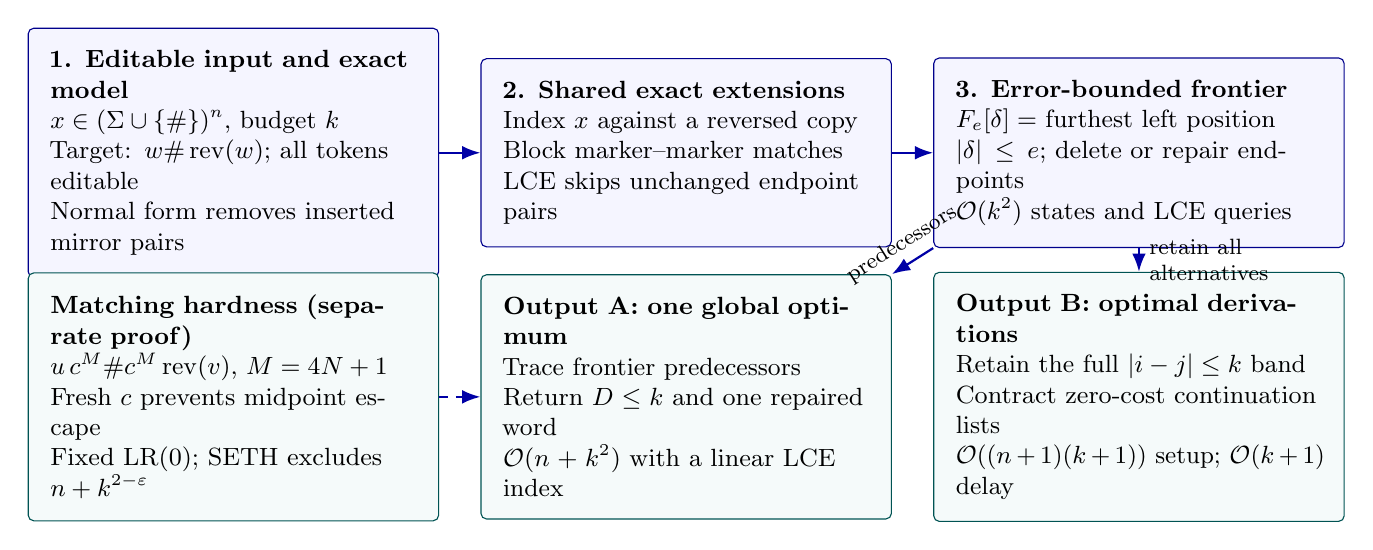
\begin{tikzpicture}[font=\small,>=Latex,
 box/.style={draw=blue!55!black,fill=blue!4,rounded corners=2pt,align=left,text width=4.65cm,inner sep=8pt,minimum height=1.72cm},
 resultbox/.style={box,draw=teal!65!black,fill=teal!4},
 arr/.style={->,thick,draw=blue!65!black}]
\node[box] (input) at (0,0) {\textbf{1. Editable input and exact model}\\$x\in(\Sigma\cup\{\#\})^n$, budget $k$\\Target: $w\#\rev(w)$; all tokens editable\\Normal form removes inserted mirror pairs};
\node[box] (index) at (5.75,0) {\textbf{2. Shared exact extensions}\\Index $x$ against a reversed copy\\Block marker--marker matches\\LCE skips unchanged endpoint pairs};
\node[box] (front) at (11.5,0) {\textbf{3. Error-bounded frontier}\\$F_e[\delta]=$ furthest left position\\$|\delta|\le e$; delete or repair endpoints\\$\Oh(k^2)$ states and LCE queries};
\node[resultbox] (lower) at (0,-3.1) {\textbf{Matching hardness (separate proof)}\\$u\,c^M\#c^M\rev(v)$, $M=4N+1$\\Fresh $c$ prevents midpoint escape\\Fixed LR(0); SETH excludes $n+k^{2-\eps}$};
\node[resultbox] (one) at (5.75,-3.1) {\textbf{Output A: one global optimum}\\Trace frontier predecessors\\Return $D\le k$ and one repaired word\\$\Oh(n+k^2)$ with a linear LCE index};
\node[resultbox] (all) at (11.5,-3.1) {\textbf{Output B: optimal derivations}\\Retain the full $|i-j|\le k$ band\\Contract zero-cost continuation lists\\$\Oh((n+1)(k+1))$ setup; $\Oh(k+1)$ delay};
\draw[arr] (input) -- (index);
\draw[arr] (index) -- (front);
\draw[arr] (front.south west) -- node[above,sloped,font=\footnotesize]{predecessors} (one.north east);
\draw[arr] (front) -- node[right,font=\footnotesize,align=left]{retain all\\alternatives} (all);
\draw[arr,dashed] (lower.east) -- (one.west);
\end{tikzpicture}
\Description{A six-box diagram shows editable marked-mirror input, a longest-common-extension index, and a two-ended error frontier. The frontier yields one optimal repair or feeds a larger band graph for enumerating optimal normal-form derivations. A guarded string-edit reduction supplies the separate conditional lower bound.}
\caption{\krepair{} for marked mirrors. $i,j$ count consumed symbols from the two ends and $\delta=i-j$; $N=\max(|u|,|v|,1)$. Solid arrows are algorithmic dependencies; the dashed arrow is a conditional lower bound. The framework does not assert compression of arbitrary LR stacks, and Output B enumerates derivations rather than distinct repaired strings.}
\label{fig:framework}
\end{figure*}

\section{Preliminaries and a Deterministic-Stack Barrier}
An edit alignment is a monotone alignment of two strings, with unequal symbol pairs and symbol--gap pairs each costing one. We freely use its equivalence to unit Levenshtein edit scripts. Reversal preserves this distance. An erasing homomorphism that sends each terminal either to itself or to the empty word cannot increase edit distance: apply the homomorphism to every alignment column and discard empty--empty columns. The triangle inequality follows by concatenating edit scripts. Empty input is permitted, and $\LED_{\Pal_\Sigma}(\eps)=1$.

\begin{lemma}[The grammar is LR(0)]\label{lem:lr}
For every finite nonempty $\Sigma$, the displayed grammar $G_\Sigma$, not just its language, is LR(0).
\end{lemma}
\begin{proof}
Augment it with $S'\to S$. Apart from the initial state and the accepting state, its canonical LR(0) item sets have the following forms: the closure of $S\to c\mathbin\cdot S c$ for each $c$; the singleton $S\to\#\mathbin\cdot$; the singleton $S\to cS\mathbin\cdot c$ for each $c$; and the singleton $S\to cSc\mathbin\cdot$ for each $c$. The closure in the first form adds all items $S\to\mathbin\cdot dSd$ and $S\to\mathbin\cdot\#$. Taking a goto on an ordinary terminal returns a closure of the first form, on $\#$ returns the marker reduction state, and on $S$ returns the corresponding state expecting $c$. Every reduction state contains one completed item and no shift item. All other nonaccepting states contain no completed item. The accepting state has only $S'\to S\mathbin\cdot$. Hence there is no shift/reduce or reduce/reduce conflict.
\end{proof}

A direct recognizer pushes ordinary symbols until $\#$ and then pops matching symbols. This is a one-turn deterministic pushdown computation. It is \emph{not} a visibly pushdown automaton under the usual fixed input-alphabet partition: the same terminal can cause a push before $\#$ and a pop after it. Deterministic, one-turn, and visibly pushdown are different restrictions.

\begin{proof}[Proof of Theorem~\ref{thm:barrier}]
Choose a set $T$ of $k$ positions among the $m$ input positions. Substitute $b$ for the symbols of $a^m$ at positions in $T$, obtaining $w_T$. A recognizer has then stored the corresponding prefix information. Give it zero remaining edit budget. The continuation $\#\rev(w_T)$ is accepted after $w_T$ and rejected after every different $w_U$: the grammar generates exactly one reversal for a given left half. Thus the configurations have distinct zero-budget continuation languages. There are $\binom{m}{k}$ choices. Already $k=1$ gives $m$ equivalence classes for a fixed grammar, contradicting any bound depending only polynomially on $k$ and $|G|$ for this equivalence relation.
\end{proof}

Each $w_T$ differs from the original prefix in only $k$ isolated symbols and has at most $k+1$ unchanged runs. The number of runs therefore gives a compact \emph{description of one configuration}; it does not count how many descriptions exist. Positions and replacement values still carry information. An error-bounded graph-structured stack could share common structure, but a proof must bound the total shared representation and justify its query operations. Continuation equivalence alone cannot supply that bound.

For general CFGs, the $k=0$ decision problem is simply membership, whereas the parse-information task can be stronger. Lee's reduction~\cite{lee2002} converts an $\Oh(g n^{3-\eps})$ general CFG parser into an $\Oh(m^{3-\eps/3})$ Boolean matrix multiplication algorithm; the grammar varies and encodes the matrices. We do not replace its parsing oracle by one fixed-grammar membership query, or infer a contradiction merely from polynomial grammar factors. Such replacements would change the theorem's quantifiers.

\section{A Normal Form for Unrestricted Marker Repair}\label{sec:normal}
Let $x[0..n)$ be the input and $\rho(s,t)=\min_{c\in\Sigma}(\ind{s\ne c}+\ind{t\ne c})$. Thus $\rho$ is zero for equal ordinary symbols, one for unequal symbols with at least one ordinary endpoint, and two when both endpoints are markers. The minimizing terminal is an endpoint that belongs to $\Sigma$, or an arbitrary fixed terminal when both endpoints are markers.

\begin{lemma}[Insertion-free mirror pairs]\label{lem:normal}
There is an optimal alignment to $\Pal_\Sigma$ in which every noncentral output symbol is aligned to a source symbol. The only possibly inserted output symbol is the central marker.
\end{lemma}
\begin{proof}
Consider a mirror pair of output symbols $c,c$. If both are inserted, remove both from the output and their alignment columns. The result is still a marked palindrome and its alignment costs two less. If exactly one is inserted and the other is aligned to source symbol $s$, remove both output symbols, replace the alignment column involving $s$ by a deletion of $s$, and discard the inserted column. The old cost on these columns was $1+\ind{s\ne c}$, whereas the new cost is one. No other alignment column changes; removing a matching outer or inner mirror pair preserves membership. Repeat until no noncentral output insertion remains. The transformation never raises cost, so applied to an optimum it gives an optimum of the required form.
\end{proof}

The lemma asserts existence of an optimal normal form. It does not assert that all optimal repaired strings survive normalization. For example, consider $a\#$: both $\#$, by deleting $a$, and $a\#a$, by inserting $a$, cost one. Only the former is in normal form.

For an interval $x[i..r)$ let $T(i,r)$ denote its distance to $\Pal_\Sigma$. The normal form gives
\begin{align}\label{eq:interval}
T(i,r)=\min\{&1+T(i+1,r),\ 1+T(i,r-1),\notag\\
             &\rho(x[i],x[r-1])+T(i+1,r-1)\},\qquad r-i\ge2,
\end{align}
with $T(i,i)=1$ and $T(i,i+1)=\ind{x[i]\ne\#}$. The three choices delete the left endpoint, delete the right endpoint, or repair both endpoints into an equal ordinary pair. On a singleton, replacing its symbol by $\#$ is never worse than deleting it and inserting $\#$.

\begin{lemma}[Exact interval recurrence]\label{lem:interval}
Equation~\eqref{eq:interval} computes the unrestricted unit LED and a minimum repaired string in $\Oh(n^2)$ time and space for fixed $\Sigma$.
\end{lemma}
\begin{proof}
Each option extends an inner solution into a valid marked palindrome at the stated cost. For the reverse inequality, take an optimal alignment in the normal form of Lemma~\ref{lem:normal}. If a source endpoint is deleted, remove that deletion and solve the remaining interval. Otherwise both endpoints are aligned to output symbols. By monotonicity, they align to the first and last noncentral output symbols, which are an equal mirror pair. If there is no such pair, the output is $\#$, and at least one endpoint is deleted when the source length is at least two. Thus one of the recurrence cases applies. Induction on interval length proves equality, including the empty and singleton bases. The table has $\Oh(n^2)$ entries and constant work per entry; predecessor traceback constructs a witness.
\end{proof}

Deleting instead of inserting a mirror endpoint is a property of the optimization over the whole target language. It is not a claim that insertions are unnecessary in string edit distance or in arbitrary CFG repair.

\section{The Error-Bounded Two-Ended Frontier}\label{sec:algorithm}
Use coordinates $(i,j)$ for the numbers of symbols consumed from the left and the right, leaving $x[i..n-j)$. A deletion moves to $(i+1,j)$ or $(i,j+1)$ at cost one. Repairing an endpoint pair moves to $(i+1,j+1)$ at cost $\rho(x[i],x[n-1-j])$, provided at least two symbols remain. Vertices satisfy $i,j\ge0$ and $i+j\le n$. An interval of length zero has completion cost one, and one of length one has completion cost $\ind{x[i]\ne\#}$. A completed interval is connected to an accepting sink at that cost.

Let $\operatorname{ext}(i,j)$ repeatedly consume a zero-cost pair until a mismatch, a marker, or an interval of length at most one remains. This extension does not consume $\#$ as an ordinary mirror symbol. It preserves $\delta=i-j$.

\begin{lemma}[LCE implementation]\label{lem:lce}
After $\Oh(n)$ deterministic preprocessing for a fixed alphabet, an extension is available in constant time. Comparison-sort preprocessing can instead be used with $\Oh(n\log^2(n+2))$ time and $\Oh(n\log(n+2))$ space.
\end{lemma}
\begin{proof}
Index $x\,\$\,y$, where $y$ is $\rev(x)$ with each marker replaced by another fresh terminal $\dagger$. Neither fresh terminal is in the input alphabet. A query between position $i$ in $x$ and position $j$ in $y$ matches exactly the ordinary endpoint pairs, stopping even on a marker--marker comparison. Cap its answer at $\lfloor(n-i-j)/2\rfloor$. Standard suffix-tree or suffix-array LCE preprocessing gives the first bound on a fixed alphabet~\cite{gusfield1997}. For the elementary alternative, prefix doubling with comparison sorting takes $\Oh(n\log^2(n+2))$ time. Kasai-style adjacent LCP computation is linear; a sparse range-minimum table takes $\Oh(n\log(n+2))$ preprocessing and space and answers each LCP query in constant time.
\end{proof}

For budget $e$ and diagonal $\delta$, $F_e[\delta]$ stores the greatest left coordinate of a retained reachable vertex after extension. Undefined entries have value $-\infty$. The entries use \emph{at most} $e$ paid edits; carrying the previous layer is therefore allowed. For a vertex on diagonal $\delta$, its right coordinate is $F_e[\delta]-\delta$. The candidate transitions are:
\begin{enumerate}
\item carry $F_{e-1}[\delta]$;
\item delete left from diagonal $\delta-1$ in layer $e-1$, giving left coordinate $F_{e-1}[\delta-1]+1$;
\item delete right from diagonal $\delta+1$ in layer $e-1$, giving $F_{e-1}[\delta+1]$;
\item repair a pair from diagonal $\delta$ in layer $e-c$, for $c\in\{1,2\}$, when its actual pair cost is at most $c$, giving $F_{e-c}[\delta]+1$.
\end{enumerate}
We discard geometrically invalid candidates and apply extension to the largest remaining coordinate. Layer zero starts at $(0,0)$ and is extended. Every retained terminal vertex gives a feasible answer by adding its center cost. We keep the smallest such answer over all processed layers, rather than returning immediately on a paid-center candidate: a free center found in the next layer may tie or improve a previously observed bound.

\begin{lemma}[Frontier dominance]\label{lem:dominance}
The retained frontiers and their terminal-completion bounds suffice to obtain a globally minimum sink distance. Discarding a smaller reachable coordinate on a fixed budget and diagonal cannot eliminate every optimum.
\end{lemma}
\begin{proof}
First observe a geometric fact: if two vertices $p\le q$ lie on the same diagonal, then extending $p$ either stops before $q$, or passes through $q$ and stops no later than the extension from $q$. Therefore the extension operator is monotone in its starting coordinate.

Consider the first paid edge of a candidate path after a vertex discarded in favor of a further vertex on the same diagonal. Carrying is harmless. A left or right deletion is available at the further vertex if its interval is nonempty; it reaches the same next diagonal at least as far as the deletion from the earlier vertex. Extension preserves that inequality. If the further interval is empty, finishing it costs one, no more than the discarded path's next paid edge. Thus replacing the remainder by immediate completion cannot increase the total cost.

For a pair edge, let $p<q$ be the earlier and further left coordinates at its predecessor budget. If the same cost allowance $c$ is legal at $q$, the pair edge and monotonicity again give dominance. The only nonterminal obstruction is a cost-one allowance at $q$ whose endpoints are both markers, since every pair costs at most two. In that case $p+1\le q$. The earlier cost-one edge, even after extension, cannot pass the already extended $q$: extension starting at or before $q$ stops no later than extension at $q$, and $q$ is already a stopped vertex. The carry candidate in the next budget layer therefore dominates it. If $q$ has fewer than two remaining symbols, finishing costs at most one, again no more than the discarded positive pair edge. Cost-two allowances never face a pair-cost obstruction.

These replacements can be applied in increasing budget order to the prefixes of an optimal path. Zero-cost extensions can always be taken using the monotonicity argument; a replacement reaching the boundary can finish immediately as just proved. Each replacement either preserves a frontier representative at least as far on the required diagonal, or produces a sink path of no larger cost. Conversely all retained transitions and completions are feasible paths in the exact interval graph. Hence the minimum observed sink distance equals the true minimum.
\end{proof}

\begin{algorithm}[t]
\caption{\krepair{} for marked mirrors}
\label{alg:frontier}
\begin{algorithmic}[1]
\Require Input $x$, threshold $k$, fixed ordinary alphabet $\Sigma$
\State Build the blocked-marker LCE index; $B\gets k+1$
\For{$e=0,1,\ldots,k$}
  \For{$\delta=-e,-e+1,\ldots,e$}
    \State Collect feasible carry, deletion, and pair candidates
    \State Include $(0,0)$ if $(e,\delta)=(0,0)$
    \If{at least one candidate exists}
      \State Extend the furthest candidate; store $F_e[\delta]$
      \State Store its predecessor and endpoint edit choice
      \If{at most one source symbol remains}
        \State $B\gets\min(B,e+\text{center completion cost})$
      \EndIf
    \EndIf
  \EndFor
\EndFor
\If{$B>k$} \State \Return ``distance exceeds $k$''
\Else \State \Return $B$ and a predecessor-traced repaired word
\EndIf
\end{algorithmic}
\end{algorithm}

\begin{proof}[Proof of Theorem~\ref{thm:upper}]
By Lemma~\ref{lem:interval}, the grid plus the accepting sink exactly represents LED. Lemma~\ref{lem:dominance} proves that Algorithm~\ref{alg:frontier} preserves its minimum sink distance. Each diagonal-changing edge costs one, so every vertex reachable within budget $e$ satisfies $|\delta|\le e$. There are $\sum_{e=0}^k(2e+1)=(k+1)^2$ possible entries. Each considers a constant number of candidates and uses at most one LCE query. Pair costs and a minimizing terminal are computable in constant time from the endpoint types. Predecessor storage uses $\Oh((k+1)^2)$ space.

Trace the predecessor of the best terminal and undo any carry steps. Nonzero pair edges choose the stored terminal, zero-cost runs copy their left source substring, and deletions emit nothing. Concatenate these contributions into the output half $w$, then return $w\#\rev(w)$. The endpoint choices and deletions also yield a source-position edit script, inserting or substituting the central marker as indicated. The normal form has no noncentral insertion, so the output length is at most $n+1$ and materialization is linear. The selected path costs at most its recorded budget plus center cost. If it cost less than the optimum, it would contradict Lemma~\ref{lem:interval}; hence it is optimal. Combine the frontier cost with Lemma~\ref{lem:lce}. Empty input and $k=0$ are handled by the explicit center rules.
\end{proof}

The furthest frontier is sufficient for one optimum, not for preserving all ties. For instance, an equal run can contain many different optimal deletion positions. Their resulting configurations need not be represented by the one furthest witness.

\section{A Correct Fixed-Grammar Lower Bound}\label{sec:lower}
The central marker is a token, so its location can change. In particular, for $u=\texttt{aaabbb}$ and $v=\texttt{bbbaaa}$,
\begin{equation}\label{eq:counter}
 \ED(u,v)=6,\qquad
 \LED_{\Pal_{\{a,b\}}}(u\#\rev(v))\le5.
\end{equation}
Deleting the three final \texttt{b}'s from \texttt{aaabbb\#aaabbb}, deleting its original marker, and substituting the remaining central \texttt{b} by \texttt{\#} gives \texttt{aaab\#baaa}. These five edits already refute equality; the exact interval oracle also gives distance five. For completeness, any alignment of $a^3b^3$ with $b^3a^3$ can match only one letter type: matching both would reverse the order of those matches. If it has $r$ matches of that type, the displacement at its first $a$ match, or last $b$ match, forces at least $r$ gaps in one direction. Equal input lengths imply the same number $g$ of gaps in both directions. Its cost is $6-r+g\ge6$, attained by six substitutions. An even simpler unequal-length family is $u=a^{2r}$, $v=\eps$: deleting the final marker and inserting one between the two $a^r$ blocks costs two, whereas $\ED(u,v)=2r$. Thus the unguarded map can lose an arbitrarily large multiplicative factor.

\begin{lemma}[Protected-marker identity]\label{lem:protected}
If the unique input marker in $u\#\rev(v)$ must align to the unique output marker, the minimum repair cost is exactly $\ED(u,v)$.
\end{lemma}
\begin{proof}
For a target $w\#\rev(w)$, the marker constraint splits the alignment and its cost into $\ED(u,w)+\ED(v,w)$. The minimum is at least $\ED(u,v)$ by the triangle inequality and is attained at $w=u$. This is a statement about a constrained alignment model, not unrestricted LED.
\end{proof}

We enforce the needed separation without protecting any symbol. Add one fresh ordinary terminal $c$ to the binary alphabet and let $N=\max(|u|,|v|,1)$.

\begin{lemma}[Guarded unrestricted identity]\label{lem:guard}
For $M=4N+1$ and $z=u\,c^M\#c^M\rev(v)$,
\begin{equation}\label{eq:guard}
 \LED_{\Pal_{\{a,b,c\}}}(z)=\ED(u,v).
\end{equation}
The map has linear time and output length $\Oh(N)$.
\end{lemma}
\begin{proof}
Let $d=\ED(u,v)\le N$. Repairing $v$ into $u$ on the reversed right core yields the valid target $u c^M\#c^M\rev(u)$ at cost $d$. Hence an optimal alignment has cost $t\le N$. Write its target as $w\#\rev(w)$, with $h=|w|$. Length difference gives
\[
 |2h-(2M+|u|+|v|)|\le t,
 \qquad h\ge M-N/2.
\]
Every prefix of a cost-$t$ alignment has input/output coordinate discrepancy at most $t$, because only insertions and deletions change that discrepancy. Cut the alignment immediately before its central output marker, at output coordinate $h$, and immediately after it, at $h+1$. Both source cuts lie within $t$ of these output coordinates. They are strictly after the left core $u$: $h-t\ge M-3N/2>N\ge|u|$. They are strictly before the right core $\rev(v)$, since
\[
 h+1+t\le M+(|u|+|v|)/2+1+3t/2
          < |u|+2M+1.
\]
The latter strict inequality follows from $|v|-|u|\le N$, $t\le N$, and $M=4N+1$. Thus the source on the left of the first cut consists of $u$ followed only by guard symbols and possibly the original marker; the source after the second cut consists only of such symbols followed by $\rev(v)$. Any source symbol consumed in the central output column is also a guard symbol or the original marker. This conclusion includes deletion columns at a cut: their source coordinates obey the same discrepancy bound.

Apply the erasing homomorphism $\pi$ that removes $c$ and $\#$ and fixes $a,b$ to the two outer alignment pieces. The left piece is an alignment from $u$ to $\pi(w)$. Reversing the right piece gives an alignment from $v$ to the same $\pi(w)$. Neither projection increases cost. The central piece has nonnegative cost and contributes no binary source symbol. Consequently
\[
 \ED(u,v)\le\ED(u,\pi(w))+\ED(v,\pi(w))\le t\le d.
\]
This proves equality. The guard length is linear in $N$ and its symbol and grammar are fixed independently of the instance.
\end{proof}

\begin{proof}[Proof of Theorem~\ref{thm:lower}]
Backurs and Indyk show a SETH-based strongly subquadratic barrier for string edit distance~\cite{backurs2015}; Bringmann and K\"unnemann strengthen it to binary strings~\cite{bringmann2015}. The binary strengthening is needed here to specify the small fixed alphabet accurately. Given their binary string-edit instance $(u,v)$, construct $z$ from Lemma~\ref{lem:guard} and invoke a hypothesized threshold algorithm with budget $k=N$. Its answer is exact since the optimum is at most $N$. The running time would be $\Oh(N+N^{2-\eps})$, or linear if the second exponent is smaller than one, contradicting binary edit-distance hardness. The same argument uses $D\le N$ for a bound parameterized by the actual optimum. Lemma~\ref{lem:lr} supplies the LR(0) property of the one fixed target grammar.
\end{proof}

For any other fixed source alphabet the same guarded proof adds just one fresh ordinary terminal to the mirror grammar. Thus the original constant-alphabet Backurs--Indyk theorem alone also proves a fixed-grammar lower bound, with a larger fixed grammar. The binary refinement gives the concise three-letter version above. No part of this argument proves the lower bound for exactly $G_{\{a,b\}}$ under unrestricted marker edits.

\section{Enumerating Repairs and What an Output Means}\label{sec:enum}
Three natural outputs are different: repaired strings, edit scripts, and derivation paths. Repeated symbols create multiple optimal alignments to one string. Independent endpoint deletions may also be ordered differently in a derivation. Theorem~\ref{thm:enum} enumerates paths in the normal-form interval graph, using succinct edit events to describe them. Its delay includes time to write those events in word-RAM words. A source position occupies one word, not zero bits.

\begin{proof}[Proof of Theorem~\ref{thm:enum}]
Retain all vertices $(i,j)$ with $i+j\le n$ and $|i-j|\le k$, plus the accepting sink. Every cost-at-most-$k$ path lies in this band. Its size is $\Oh((n+1)(k+1))$. Label pair edges by their chosen terminal, keeping all cost-minimizing choices, and retain deletions and center-completion edges. There are constantly many edges per vertex for fixed $\Sigma$. A pair choice of nonminimum cost for that same endpoint pair cannot occur on a globally optimal path, since replacing the chosen terminal by a minimizing one changes no inner subproblem and lowers the total cost.

The graph is acyclic: all nonsink edges consume a source symbol. Compute source distances $f$ and sink distances $b$ in topological order, and let $D$ be the source-to-sink distance. Retain only edges $(p,q)$ with weight $\omega$ satisfying $f(p)+\omega+b(q)=D$. Such edges are tight: since $f(q)\le f(p)+\omega$ and $D\le f(q)+b(q)$, equality forces $f(q)=f(p)+\omega$. Every source-to-sink path in the retained graph therefore has total cost $D$, and every optimum remains.

A vertex has at most one zero-cost outgoing edge. It is either the unique unchanged ordinary pair or a zero-cost central-marker completion. Process vertices backwards. For each vertex $p$, construct a persistent option list containing its positive-cost tight outgoing edges, followed by the option list of its zero-cost successor if one exists. A zero-cost path to the sink contributes a special finish option. Each vertex contributes only its own constant number of list cells; the inherited tail is shared. The lists therefore take linear time and space in the band size, even when the same free run is visible from many vertices.

Depth-first enumeration now chooses one list option at a time. A positive-cost option specifies a particular edge after a uniquely determined sequence of zero-cost edges; it recurses from that edge's target. A finish option emits the current event sequence. Every recursion step spends at least one unit, so depth is at most $D\le k$. Each list contains only options with an optimal completion, so no explored branch is fruitless. Between consecutive outputs the traversal backs up at most $k$ levels and descends at most $k$ levels. This proves $\Oh(k+1)$ worst-case delay, including the first output and termination. Each positive pair edge emits one or two substitutions, deletion emits one deletion, and a paid center emits one insertion or substitution. The event count is the path cost, at most $k$. The option choices reconstruct a unique outer-to-inner graph path; paths with different edit order remain distinct derivations. The preprocessing and space bounds follow from the band size.
\end{proof}

Normal-form existence does not justify reporting these outputs as \emph{all distinct minimum repaired strings}. The example $a\#$ from Section~\ref{sec:normal} loses the optimal output $a\#a$ under normalization. Recovering every output requires preserving insertion choices too, as well as removing duplicates. A general but slower construction gives a clean existence guarantee.

\begin{proposition}[Distinct repaired strings]\label{prop:strings}
Given a CFG $G$ over a finite alphabet, input $x$, and threshold $k$, all distinct globally minimum repaired strings can be enumerated without repetition with preprocessing and delay polynomial in $n,k,|G|$, and the alphabet size. No polynomial dependence only on $k,|G|$ is asserted.
\end{proposition}
\begin{proof}
Build the edit-neighborhood NFA over \emph{output} symbols with states $(i,e)$, $0\le i\le n$, $0\le e\le k$. Inserting an output symbol advances $e$; matching or substituting consumes one input symbol and reads one output symbol, advancing $e$ by zero or one; deleting an input symbol is an epsilon transition advancing both $i$ and $e$. Initial state is $(0,0)$ and accepting states are $(n,e)$ with $e\le k$. This NFA recognizes exactly the strings within distance $k$ of $x$, each of length at most $n+k$.

For each budget $d=0,\ldots,k$, intersect the NFA for budget $d$ with $G$. CFG--NFA intersection and emptiness take polynomial time. Explicitly, after epsilon elimination and grammar binarization, product nonterminals are $[p,A,q]$ and a binary production $A\to BC$ introduces $[p,A,q]\to[p,B,r][r,C,q]$ for each middle state $r$. Terminal rules use NFA transitions. The product size is polynomial, and productivity is a finite fixed-point computation. The first nonempty product gives the minimum $d=D$; if none is nonempty, report $D>k$.

For a prospective output prefix $p$, also intersect with a DFA for $p\Sigma^*$. Its size is $\Oh(|p|+2)$. The same emptiness construction decides whether any minimum repaired string extends $p$. Traverse the prefix trie, asking this oracle before descending. Report a node itself exactly when its word belongs to $L(G)$ and has distance $D$ from $x$. Empty prefixes and empty repaired words are included. Depth is at most $n+D$. Between outputs, depth-first traversal tests at most $\Oh((|\Sigma|+1)(n+k+1))$ candidate prefixes, each of polynomial size. Every successful subtree has an output, and every output has a unique prefix path, so delay is polynomial and no repaired string is repeated. For an explicit crude bound, the product uses $\Oh((n+1)(k+1)(n+k+2))$ automaton states before grammar intersection; the cubic product construction already suffices.
\end{proof}

Printing a length-$\Theta(n)$ repaired word requires $\Omega(n)$ symbol-output time even when $k=0$. Allowing large preprocessing does not remove this output cost. A proposed $\operatorname{poly}(k,|G|)$ delay statement must therefore use a succinct representation or add output length to the bound. Proposition~\ref{prop:strings} handles literal strings and includes that dependence.

\section{Weighted Costs}\label{sec:weights}
The unit-cost frontier should not be generalized by changing a few constants. When deletion cost depends on its symbol, an affordable deletion at an earlier vertex on a diagonal need not be affordable at a later vertex. The key dominance proof for that edge then fails.

A complete quadratic extension is available under a useful explicit cost model. Let $\gamma$ be a symmetric metric on $\Sigma\cup\{\#,\eps\}$, where the distinguished $\eps$ represents a gap rather than an input token. Match cost is zero, insertion/deletion of $c$ costs $\gamma(c,\eps)$, and substitution $c\to d$ costs $\gamma(c,d)$. Distinct points have positive cost, and arithmetic on costs is assumed constant-time; otherwise the appropriate bit complexity must be included.

\begin{proposition}[Metric-weighted mirrors]\label{prop:weighted}
For this symmetric metric cost model, LED to $\Pal_\Sigma$ and an optimal witness can be computed in $\Oh(|\Sigma|n^2)$ time and $\Oh(n^2)$ space, after receiving the cost table. The input and marker are unrestricted.
\end{proposition}
\begin{proof}
For a pair with one inserted endpoint $c$ and one endpoint aligned to $s$, deleting the pair and deleting $s$ costs $\gamma(s,\eps)$ instead of $\gamma(s,c)+\gamma(c,\eps)$. The triangle inequality makes the replacement nonincreasing. A doubly inserted pair can still be removed. Thus Lemma~\ref{lem:normal} holds. In the interval recurrence, replace left and right unit costs by $\gamma(x[i],\eps)$ and $\gamma(x[r-1],\eps)$, and replace $\rho$ by $\min_{c\in\Sigma}(\gamma(x[i],c)+\gamma(x[r-1],c))$. Empty intervals cost $\gamma(\eps,\#)$; singleton intervals cost $\gamma(x[i],\#)$, since delete-plus-insert cannot be cheaper by the triangle inequality. The proof of Lemma~\ref{lem:interval} then applies verbatim with these costs. Scanning the ordinary alphabet per interval gives the stated bound, and predecessor choices give a witness.
\end{proof}

For arbitrary asymmetric or nonmetric costs, the normal-form inequality need not hold. General weighted error-correcting parsing remains a valid fallback when costs are nonnegative and appropriately encoded, but Proposition~\ref{prop:weighted} does not claim its quadratic or additive bound. Even for two strings, bounded weighted edit distance has a substantially different algorithmic landscape~\cite{cassis2023}. Positive lower bounds on edit cost are also necessary when a cost budget is used to bound output length; zero-cost insertions can create infinitely many optimal repairs.

\section{Executable Verification and Compiler Evaluation}\label{sec:verification}
The executable artifact contains an independent interval oracle, a direct finite-language oracle, a scan-based frontier, and a suffix-indexed implementation that returns an actual repair. The finite-language oracle is independent of the normal-form recurrence: it enumerates candidate halves and computes their ordinary string-edit distances. Its search is finite and complete because the incumbent distance to $\#$ bounds the length of every candidate that could improve that incumbent. These are correctness checks of the restricted mathematical model, not measurements of a compiler recovery system.

\begin{table}[t]
\caption{Executed verification checks. Each number counts completed comparisons or witnesses; no row is a projected benchmark. All comparisons passed.}
\label{tab:checks}
\small
\begin{tabularx}{\columnwidth}{@{}X r@{}}
\toprule
Check family & Checks\\
\midrule
Interval oracle vs. explicit target-language enumeration; $|x|\le6$, alphabet $\{a,b,\#\}$ & 1,093\\
Scan frontier vs. interval oracle; $|x|\le9$, several thresholds & 177,086\\
Guarded identity; all binary cores of length at most four & 961\\
Randomly corrupted ternary mirrors; five thresholds per input & 2,500\\
Indexed frontier: threshold answers and returned witnesses; $|x|\le7$, $k\in\{0,1,2,3,4\}$ & 16,400\\
\bottomrule
\end{tabularx}
\end{table}

The first test covers all 1,093 source strings of length at most six over $\{a,b,\#\}$. The second covers every such string of length at most nine and budgets from zero through $\min(|x|+1,5)$, giving 177,086 threshold comparisons. The guard test covers the 31 binary words of length at most four in both argument positions, giving 961 pairs. Random tests use a recorded deterministic seed and 500 independently generated ternary mirrors, followed by random edit sequences; they compare five budgets per resulting input against the interval oracle. The indexed implementation is checked on 16,400 threshold instances, including independent string-edit verification of every returned witness. The code and machine-readable logs preserve the exact parameters. These finite checks support implementation consistency; the proofs, not the tested bounds, establish correctness on all inputs.

The implementation is dependency-free Python. Its suffix-array construction uses comparison sorting and its LCP queries use a sparse RMQ table, matching the elementary implementation bound in Theorem~\ref{thm:upper}. We do not infer a near-linear measured runtime from the separate scan-based verifier. The artifact does not contain a Rust integration with grmtools, lrpar, or tree-sitter, and does not claim speedups over those systems.

\subsection{What would establish programmer-intent agreement}
A compiler study must distinguish at least three events: a returned token sequence parses; its edit cost is globally minimum; and its text or tokens agree with a recorded human fix. These are not interchangeable success definitions. For paired broken/human-fixed files $(x_i,h_i)$ under one tokenizer and grammar, useful exact metrics are
\begin{align*}
 H_{\mathrm{min}}&=\frac{1}{m}\sum_i\ind{h_i\in L(G),\ \ED(x_i,h_i)=D_i},\\
 H_{\mathrm{top}}&=\frac{1}{m}\sum_i\ind{\widehat h_i=h_i},
 \qquad D_i=\LED_G(x_i).
\end{align*}
$H_{\mathrm{min}}$ asks whether the observed human fix is one of the minima; $H_{\mathrm{top}}$ asks whether a particular ranking returns it. If only the human edit cost is known, minimum status requires an exact certificate or lower bound; successful parsing alone is insufficient. Uncertified cases must be reported as such rather than silently counted as failures or successes. Multiple-file edits, lexical changes, indentation tokens, identifier spellings, and formatting normalization must be fixed in the experimental definition.

CPCT+'s published Blackbox evaluation uses 200,000 invalid Java programs and reports $98.37\%\pm0.017\%$ repaired within a $0.5$-second timeout~\cite{cpct2020}. Seq2Parse reports evaluation on a 1.1-million-program Python dataset, parsing 94\% of its tests within 2.1 seconds and producing the exact user fix in about one third of cases~\cite{seq2parse2022}. These are source-reported results with different protocols, not reruns or entries in a common leaderboard. An invalid-file corpus alone also does not supply the human-fix pairing required for $H_{\mathrm{min}}$.

A direct evaluation of a future general-LR algorithm should pair Java Blackbox histories and student Python revisions with an exact tokenizer specification, pin grammar and baseline revisions, and use identical resource limits. CPCT+, tree-sitter recovery, Burke--Fisher-style recovery, Seq2Parse, and a specified LLM can be compared on parsing success, exactness certificates, human agreement, and per-file runtime. Local recovery and partial parse-tree production require separate reporting from whole-file repair. A learned or language-model baseline additionally needs model version, prompt, decoding policy, and training-data exclusions. None of these missing compiler experiments is assigned an inferred numerical result here.

For the proposed skeleton method, informative ablations would retain all configurations, use shared stack fragments, and then add continuation-safe dominance; changing only an implementation flag without a proved summary invariant would not test the theoretical claim. Adversarial families should vary error locations, common-prefix length, nesting, and grammar size, as well as $k$. The binomial family of Theorem~\ref{thm:barrier} is a specific stress test for explicit continuation-equivalence classes. Such a study is additional work, because the present mirror algorithm does not implement general-LR recovery.

\section{The Remaining General-LR Question}\label{sec:open}
An arbitrary LR(1) parser can perform long reduction sequences after one token change, and two configurations with the same input offset can have different legal continuations. An LCE of the remaining token strings does not certify an equal parser execution. A valid generalization of \krepair{} needs a configuration-aware extension primitive and a dominance relation preserved by all future edits. Theorem~\ref{thm:barrier} excludes one natural candidate relation, while leaving implicit representations open.

\begin{conjecture}[General deterministic repair]\label{conj:lr}
After an explicit polynomial-size deterministic parser representation is supplied, threshold LED for an LR(1) grammar admits a bound of the form $\softO(n\operatorname{poly}(|G|)+\operatorname{poly}(k,|G|))$, or at least $n\operatorname{poly}(k,|G|)$.
\end{conjecture}

The parser representation matters. A bound polynomial in the number of source productions is not automatically polynomial in the size of a canonical LR(1) table, which may be much larger. The conjecture deliberately does not hide parser construction in a linear input scan. We neither prove nor refute either bound for arbitrary LR(1) grammars. In particular, an $n^{k+1}$ search over edit positions, while exact, would not establish the stated fallback bound.

For visibly pushdown languages, a fixed partition tells whether an input symbol pushes, pops, or leaves the stack unchanged. Edits can still alter that partition action, and arbitrary finite-state restrictions on nesting remain relevant. The general Dyck algorithm does not directly repair to every regular restriction of a Dyck language: a closest balanced string may violate that restriction. Conversely, the marked-mirror theorem here is not a theorem for all visibly pushdown languages. A transfer theorem must preserve both accepted structure and edit cost, rather than rely on informal similarity to a programming language grammar.

The proved results give a quadratic, conditionally tight parameter dependence for a fixed deterministic subclass with fully editable markers. They also identify three obligations for a broader syntax-repair theorem: continuation-safe compression, marker-safe lower-bound gadgets, and output-sensitive enumeration. The universal LR(1) upper bound and a real-code measurement of minimum-versus-human repair agreement remain separate unresolved objectives.

\balance
\makeatletter\@ACM@balancefalse\makeatother
\bibliographystyle{ACM-Reference-Format}
\bibliography{references}
\end{document}
